\documentclass[letterpaper,10pt]{article}
\usepackage[utf8]{inputenc}
\usepackage{graphicx}
\usepackage{caption}
\usepackage{enumitem}
\usepackage[hidelinks]{hyperref}
\usepackage{amsmath}
\usepackage{amssymb}
\usepackage{adjustbox}
\usepackage{float} 
\usepackage{wrapfig}
\usepackage{xcolor} % Para definir colores
\usepackage{listings} % Para listados de código
\usepackage{array}
\usepackage{pgfplots}


\usepackage[margin=1in]{geometry} % Agrega esta línea para establecer los márgenes
% Configuración de colores
\pgfplotsset{compat=1.18}
\definecolor{commentcolor}{rgb}{0,0.6,0}
\definecolor{stringcolor}{rgb}{0.58,0,0.82}
\definecolor{keywordcolor}{rgb}{0,0,1}
\definecolor{backcolour}{rgb}{0.95,0.95,0.92}
\definecolor{grisclaro}{rgb}{0.9, 0.9, 0.9}
\definecolor{crtitle}{RGB}{112,48,160}
\hypersetup{
    colorlinks=true,
    linkcolor=black,
    urlcolor=blue    
}

% Configuración del estilo de los listados de código
\lstset{
    language=Go, % Define el lenguaje del código (Scala en este caso)
    basicstyle=\ttfamily\small, % Estilo de fuente básico
    commentstyle=\color{commentcolor}\ttfamily,
    stringstyle=\color{stringcolor}\ttfamily,
    keywordstyle=\color{keywordcolor}\bfseries\ttfamily,
    backgroundcolor=\color{grisclaro}, % Color de fondo
    showstringspaces=false, % No mostrar espacios en cadenas como caracteres especiales
    numbers=left, % Números de línea a la izquierda
    numberstyle=\tiny\color{gray}, % Estilo de los números de línea
    breaklines=true, % Romper líneas largas
    captionpos=b, % Posición del título ('b' para abajo)
    frame=single % Marco alrededor del código
}

\begin{document}
\begin{titlepage}
    \begin{center}
    
    
    
\includegraphics[scale=0.35]{Images/RojoTransparenteUV.png} \vspace{0.5cm}
    
    \textsc{\Large Proyecto de curso } \vspace{0.5cm} % Thesis type
    
    
    \rule{14cm}{0.05cm} \vspace{0.4cm} % Horizontal line
    
    
    \Large{\textbf{   Moderando el extremismo de opiniones en una red social  }}\vspace{0.4cm} % Thesis title
    
    \rule{14cm}{0.05cm} \vspace{1.5cm} % Horizontal line
     
    \large{\textit{realizado por:}} \\
    \Large{{\color{crtitle} 
    \textsuperscript{1}Juan Camilo Narvaez Tascón - 202140112, \\
    \textsuperscript{2}Julián Ernesto Puyo Mora - 202226905,\\
    \textsuperscript{3}Cristian David Pachecho Torres - 20222743,\\
    \textsuperscript{4}Juan Sebastián Molina Cuéllar - 202224491}
    }  %AUTHOR
    
    \vspace{2cm}
    
    \large \textit{
    Informe realizado para el curso de Análisis y Diseño de Algoritmos II,\\
    Profesor: Juan Francisco Díaz Frías - Profesor: Jesús Alexander Aranda\\
    Monitor: Mauricio Muñoz} 
    
    \vspace{0.3cm} % University requirement text
    
    \textit{de la}
    
    \vspace{0.4cm}
    
    Escuela de Ingeniería de Sistemas y Computación,\\ 
    Facultad de Ingeniería,\\ 
    Universidad del Valle
    
    \vspace{1.0cm} 
    {\color{crtitle} \small \textit{  
        \textsuperscript{1}juan.narvaez.tascon@correounivalle.edu.co, 
        \textsuperscript{2}julian.puyo@correounivalle.edu.co, 
        \textsuperscript{3}cristian.pacheco@correounivalle.edu.co,
        \textsuperscript{4}juan.sebastian.molina@correounivalle.edu.co
    }}\\
    \today
     
    
    \end{center}
    \end{titlepage}
\newpage

\tableofcontents
\newpage
\section{Introducción}
\label{sec:introduccion}
El presente informe tiene como objetivo abordar el problema de moderar el extremismo de opiniones en una red social, aplicando diferentes estrategias de diseño como fuerza bruta, algoritmos voraces y programación dinámica.

Se realizará una comparación entre estas estrategias basándose en su complejidad y optimalidad.

Para la implementación del proyecto, se ha seleccionado el lenguaje de programación \href{https://go.dev/}{Golang}. Esperamos que este informe sea de su agrado y cumpla con las expectativas del curso.
\section{Definición de estructuras y funciones útiles}
A continuación se presentan las funciones auxiliares y tipos de datos utilizados para implementar las soluciones al problema de moderar el extremismo de opiniones en la red social.
\subsection*{Tipos de datos}
A continuación, se muestran los tipos de datos definidos para representar la red social y los agentes en la misma.
\subsubsection*{Red Social}
\begin{equation}
  \mathcal{R} \mathcal{S} = < AG, R\_max >
\end{equation}\label{eq:red_social}
\begin{equation}
  AG = < a_1, a_2, \ldots, a_n >
  \label{eq:agentes}
\end{equation}
\begin{equation}
  R\_max \in \mathbb{N}
  \label{eq:recursos}
\end{equation}

Donde $AG$ es un conjunto de agentes y $R\_max$ es la cantidad máxima de recursos disponibles.

\begin{lstlisting}[caption={Definición de red social}, label={lst:r_s}]
type Network struct {
    Agents    []Agent
    Resources uint64
}
\end{lstlisting}
\subsubsection*{Agente}

\begin{lstlisting}[caption={Definición de agente}, label={lst:agente}]
type Agent struct {
    Opinion     int8
    Receptivity float64
}
\end{lstlisting}
Donde un agente $a_i$ es una pareja: $<{o_i}{^{\mathcal{R} \mathcal{S}}}, {r_i}{^{\mathcal{R} \mathcal{S}}}>$.
\newpage
\subsubsection*{Extremismo de una red $\mathcal{R}\mathcal{S}$}
\begin{equation}
  Ext(\mathcal{R}\mathcal{S}) = \frac{\sqrt{\sum_{i=0}^{n-1}{({o_i}{^{\mathcal{R} \mathcal{S}}})^2}}}{n}
  \label{eq:extremismo}
\end{equation}

\begin{lstlisting}[caption={Implementación del extremismo}, label={lst:ext}]
// extremism calculates the extremism of the network. It returns a float64 value.
func extremism(network *Network) float64 {
	var sumOpinions float64

	for _, agent := range network.Agents {
		sumOpinions += float64(agent.Opinion) * float64(agent.Opinion)
	}

	return math.Sqrt(sumOpinions) / float64(len(network.Agents))
}
\end{lstlisting}
\subsubsection*{Aplicar una estrategia de moderación $Mod(\mathcal{R}\mathcal{S},E)$}
\begin{equation}
  Mod(\mathcal{R}\mathcal{S}, E) = \mathcal{R}\mathcal{S}'
\end{equation}\label{eq:mod}
donde,
\begin{equation}
  o_i^{\mathcal{R}\mathcal{S}'} = 
  \begin{cases} 
        o_i^{\mathcal{R}\mathcal{S}'} & \text{si } e_i = 0 \\
        0        & \text{si } e_i = 1 
  \end{cases}
  \label{eq:mod_opinion}
\end{equation}

\begin{lstlisting}[caption={Implementación del Mod}, label={lst:mod}]
// moderation applies the strategy to the network. It returns the network after applying the strategy.
func moderation(network *Network, strategy []byte) *Network {
	networkPrime := Network{
		Agents:    make([]Agent, len(network.Agents)),
		Resources: network.Resources,
	}

	for i, strategyValue := range strategy {
		networkPrime.Agents[i].Opinion = network.Agents[i].Opinion - network.Agents[i].Opinion*int8(strategyValue)
	}

	return &networkPrime
}
\end{lstlisting}
\newpage
\subsubsection*{Esfuerzo}
El valor de esfuerzo a modelar la red $\mathcal{R}\mathcal{S}$.
\begin{equation}
  Esfuerzo(\mathcal{R}\mathcal{S}, E) = \sum_{i=0}^{n-1} \left\lceil  |o_i^{\mathcal{R}\mathcal{S}} - o_i^{\mathcal{R}\mathcal{S}'}| \times (1 - r_i^{\mathcal{R}\mathcal{S}}) \right\rceil
  \label{eq:esfuerzo}
\end{equation}

Donde $E$ (estrategia) es una secuencia que indica qué opinión de qué agente se modera por medio de $E$.
\begin{lstlisting}[caption={Implementación del esfuerzo}, label={lst:esfuerzo}]
  // effort calculates the effort of the network after applying the strategy. It returns a float64 value.
  func effort(network *Network, strategy []byte) float64 {
    n := len(network.Agents)
    networkPrime := moderation(network, strategy)
  
    var effortValue float64
    for i := 0; i < n; i++ {
      diff := float64(network.Agents[i].Opinion - networkPrime.Agents[i].Opinion)
      effortValue += math.Ceil(math.Abs(diff) * (1 - network.Agents[i].Receptivity))
    }
  
    return effortValue
  }
\end{lstlisting}
\section{Solución con Fuerza Bruta}
\label{sec:fuerza_bruta}

\subsection{Descripción del Algoritmo}
\label{subsec:descripcion_fuerza_bruta}
El enfoque de fuerza bruta para abordar el problema de moderar el extremismo se basa en generar todas las posibles estrategias de moderación \( E \) para una red social \( \mathcal{R}\mathcal{S} \) y seleccionar aquella estrategia que minimice el extremismo de la red social después de su aplicación, respetando la restricción de recursos \( R\_max \).

Formalmente, esto se expresa como:

\[
 AG \in \mathcal{R}\mathcal{S} \rightarrow \exists E = \langle e_0, e_1, \ldots, e_n \rangle \mid Esfuerzo(\mathcal{R}\mathcal{S}, E) \leqslant R\_max ~ \wedge ~ \min(Ext(Mod(\mathcal{R}\mathcal{S}, E)))
\]

Donde \( E \) es la estrategia de moderación aplicada a los agentes de la red social \( \mathcal{R}\mathcal{S} \), y la solución óptima es aquella que minimiza el extremismo \( Ext \) sin exceder los recursos disponibles "$\min(Ext(Mod(\mathcal{R}\mathcal{S}, E)))$".

\subsubsection*{Generación de Estrategias (StrategyGenerator)}
El primer paso es generar todas las posibles estrategias de moderación para una red social con \( n \) agentes. Para ello, se utiliza la función \( StrategyGenerator \) que genera todas las combinaciones posibles de estrategias de moderación.
\begin{lstlisting}[caption={Strategy Generator}, label={lst:strategy_generator}]
func StrategyGenerator(n int) [][]byte {
  total := 1 << n
  combinations := make([][]byte, total)
  
  for i := 0; i < total; i++ {
    combination := make([]byte, n)
    for j := 0; j < n; j++ {
      combination[n-j-1] = byte((i >> j) & 1)
    }
    combinations[i] = combination
  }

  return combinations
}
\end{lstlisting}
\textit{Esta función genera todas las posibles estrategias de moderación para una red social con \( n \) agentes. Cada estrategia es representada por una secuencia de \( n \) bits, donde el bit \( i \) indica si el agente \( i \) es moderado o no.
}
\\

\textbf{Explicación del código:}
\begin{itemize}
  \item Se inicia la función con un parametro $n$ el cual indica la cantidad de agentes de la red social, luego en la linea 2 "\textit{total := 1 $<<$ n}".
  \item Se crea un arreglo de arreglos de bytes llamado "\textit{combinations}" en la linea 3.
  \item Se inicia un ciclo for que va desde 0 hasta el total de combinaciones posibles en la linea 6.
  \item Se crea un arreglo de bytes llamado "\textit{combination}
  \item Se inicia un ciclo for que va desde 0 hasta la cantidad de agentes de la red social en la linea 7.
  \item Se asigna a la posición $n-j-1$ del arreglo de bytes "\textit{combination}" el valor de la operación $i >> j$ en la linea 8.
  \item Se asigna el arreglo de bytes "\textit{combination}" a la posición $i$ del arreglo de arreglos de bytes "\textit{combinations}" en la linea 10.
  \item Se retorna el arreglo de arreglos de bytes "\textit{combinations}" en la linea 13.
\end{itemize}
\subsubsection*{Algoritmo de Moderación (ModexFB)}
\begin{lstlisting}[caption={Algoritmo de Fuerza Bruta}, label={lst:modexfb}]
func ModexFB(network *Network) (bestStrategy []byte, bestEffort float64, minExtremism float64, err error) {
  numAgents := len(network.Agents)
  
  if numAgents > 25 {
    return nil, 0, 0, errors.New("In ModexFB the number of agents must be less than or equal to 25")
  }

  var possibleStrategies [][]byte = strategyGenerator(numAgents)
  minExtremism = math.Inf(1)
  bestEffort = math.Inf(1)
  
  for _, strategy := range possibleStrategies {
    effortValue, networkPrime := effort(network, strategy)
    if effortValue <= float64(network.Resources) {
      extremismValue := extremism(networkPrime)
      if extremismValue < minExtremism {
        minExtremism = extremismValue
        bestEffort = effortValue
        bestStrategy = strategy
      }
    }
  }
  return bestStrategy, bestEffort, minExtremism, nil
}
\end{lstlisting}
\textit{La función \textit{ModexFB} toma como parámetro un puntero a una estructura \textit{Network} y retorna la mejor estrategia (\textit{bestStrategy}), el esfuerzo asociado a dicha estrategia (\textit{bestEffort}), el extremismo mínimo alcanzado (\textit{minExtremism}), y un posible error (\textit{err}).}
\begin{itemize}
  
  \item En la línea 2, se inicializa la variable \textit{numAgents} con el número de agentes en la red social (número de elementos en \textit{network.Agents}).
  \item En la línea 4, si el número de agentes supera los 25, la función retorna un error, indicando que el número de agentes debe ser menor o igual a 25 (esto evita la explosión combinatoria al generar estrategias).
  \item En la línea 7, se llama a la función \textit{strategyGenerator} (\ref{lst:strategy_generator}) para generar todas las posibles combinaciones de estrategias de moderación, que son almacenadas en \textit{possibleStrategies}
  \item En las líneas 8 y 9, se inicializan las variables \textit{minExtremism} y \textit{bestEffort} con valores infinitos positivos (\textit{math.Inf(1)}), de forma que cualquier valor que se calcule después será menor que este valor inicial.
  \item Se inicia un ciclo \textit{for} en la línea 11 que recorre todas las estrategias generadas en \textit{possibleStrategies}.
  \item En la línea 12, se calcula el esfuerzo (\textit{effortValue}) asociado a una estrategia usando la función \textit{effort} (\ref{lst:esfuerzo}), y también se obtiene una nueva red \textit{networkPrime}, que es la red social modificada según esa estrategia.
  \item En la línea 13, se verifica si el esfuerzo es menor o igual a los recursos disponibles en la red (\textit{network.Resources}). Si es así, la estrategia es válida y se procede a calcular su nivel de extremismo.
  \item En la línea 14, se calcula el nivel de extremismo de la red modificada (\textit{networkPrime}) con la función \textit{extremism}.
  \item Si el nivel de extremismo es menor que el mínimo extremismo registrado (\textit{minExtremism}), en la línea 15 se actualizan las variables \textit{minExtremism}, \textit{bestEffort}, y \textit{bestStrategy} con los valores de la estrategia actual.
  \item Finalmente, en la línea 19, se retorna la mejor estrategia encontrada (\textit{bestStrategy}), su esfuerzo (\textit{bestEffort}), el mínimo nivel de extremismo (\textit{minExtremism}) y ningún error.
\end{itemize}

Este algoritmo de fuerza bruta genera todas las posibles estrategias de moderación y selecciona la mejor según dos criterios: esfuerzo mínimo y extremismo mínimo, siempre que el esfuerzo no exceda los recursos de la red.
\subsubsection*{ModexFB mejorado}

Debido a que el siclo realizado en la función \textit{ModexFB} (\ref{lst:modexfb}) recorre todas las estrategias posibles, además de en la línea 18 llamar a \textit{strategyGenerator} (\ref{lst:strategy_generator}) pero para evitar la exploración de estrategias inecesarias y además en el mismo recorrido calcular el esfuerzo y el extremismo de la red, se puede mejorar el algoritmo de la siguiente manera:
\begin{lstlisting}[caption={ModexFB mejorado}, label={lst:modexfb_mejorado}]
func ModexFB(network *Network) (bestStrategy []byte, bestEffort float64, minExtremism float64, err error) {
	numAgents := len(network.Agents)

	if numAgents > 25 {
		return nil, 0, 0, errors.New("In ModexFB the number of agents must be less than or equal to 25")
	}

	total := 1 << numAgents
	minExtremism = math.Inf(1)

	for i := 0; i < total; i++ {
		strategy := make([]byte, numAgents)
		for j := 0; j < numAgents; j++ {
			strategy[numAgents-j-1] = byte((i >> j) & 1)
		}
		effortValue, networkPrime := effort(network, strategy)
		if effortValue <= float64(network.Resources) {
			extremismValue := extremism(networkPrime)
			if extremismValue < minExtremism {
				minExtremism = extremismValue
				bestEffort = effortValue
				bestStrategy = strategy
			}
		}
	}

	return bestStrategy, bestEffort, minExtremism, nil
}
\end{lstlisting}
\subsection{Complejidad}
\label{subsec:complejidad_fuerza_bruta}
Para analizar la complejidad del algoritmo debemos de considerar los dos ciclos \textit{for} que ocurren dentro del código, el primer ciclo (linea 11) hace un recorrido sobre todas las posibles combinaciones de agentes que existen (linea 8 \textit{total = 1 $<<$ numAgents}), y el segundo ciclo (linea 13) hace un recorrido por el total de agentes (linea 2 \textit{numAgents:= len(network.Agents)}).

\textbf{Entonces tenemos que:}
\begin{itemize}
  \item El primer ciclo tiene una complejidad de \(O(2^n)\), debido a que $e_i$ puede tomar dos valores ($0$ o $1$) donde \(n\) es el número de agentes en la red social.
  \item El segundo ciclo tiene una complejidad de \(O(n)\), donde \(n\) es el número de agentes en la red social.
\end{itemize}
Debido a que los demás cálculos internos realizados son de complejidad \(O(1)\), la complejidad total del algoritmo es \(O(2^n \cdot n)\).
\subsection{Corrección}
\label{subsec:correccion_fuerza_bruta}
Sea $RS$ una red social con $n$ agentes $AG = \{a_1, a_2, \dots, a_n\}$.

Definimos una estrategia de moderación como un vector:

\[
E = \langle e_1, e_2, \dots, e_n \rangle
\]

donde:
\begin{itemize}
  \item $e_i \in \{0, 1\}$ para $1 \leq i \leq n$.
  \begin{itemize}
    \item $e_i = 1$: el agente $a_i$ es moderado.
    \item $e_i = 0$: el agente $a_i$ no es moderado.
  \end{itemize}
\end{itemize}

El conjunto de todas las estrategias posibles es:

\[
\mathcal{E} = \{\langle e_1, e_2, \dots, e_n \rangle \mid e_i \in \{0, 1\} \, \forall i\}
\]

\subsubsection*{Número total de estrategias posibles}

Cada agente tiene 2 opciones (ser moderado o no), y hay $n$ agentes. Por lo tanto, el número total de estrategias posibles es:

\[
|\mathcal{E}| = 2^n
\]

\subsubsection*{Análisis de la función \textit{strategyGenerator(n)} (\ref{lst:strategy_generator})}

Descripción de la función:

La función \textit{strategyGenerator(n)} (\ref{lst:strategy_generator}) genera todas las posibles combinaciones de estrategias para $n$ agentes. Lo hace de la siguiente manera:

\begin{itemize}
    \item Calcula el total de combinaciones posibles: $total = 2^n$.
    \item Itera desde $i = 0$ hasta $i = 2^n - 1$.
    \item Para cada $i$, genera una combinación binaria de longitud $n$, donde cada bit representa $e_j$ para el agente $a_j$.
\end{itemize}

\textbf{Demostración de que genera todas las estrategias}
\\

\textbf{Cobertura completa}: El rango de $i$ desde $0$ hasta $2^n - 1$ asegura que se cubren todas las posibles combinaciones binarias de longitud $n$.

\textbf{Correspondencia uno a uno}: Cada entero $i$ en este rango tiene una representación binaria única de $n$ bits. Esta representación binaria se asigna directamente a una estrategia $E = \langle e_1, e_2, \dots, e_n \rangle$, donde $e_j$ es el bit $j$ de $i$.

\textbf{Conclusión}: La función \textit{strategyGenerator(n)} (\ref{lst:strategy_generator}) genera exactamente todas las $2^n$ estrategias posibles en $E$, sin omitir ni repetir ninguna.

\subsubsection*{Funcionamiento del algoritmo \textit{ModexFB}}

\textbf{Paso a paso del algoritmo}
\\

\textbf{Generación de estrategias}:
\begin{itemize}
    \item Llama a \textit{strategyGenerator(n)} (\ref{lst:strategy_generator}) para obtener el conjunto completo de estrategias posibles $E$.
\end{itemize}

\textbf{Inicialización de variables}:
\begin{itemize}
    \item Establece \textit{minExtremism} y \textit{bestEffort} con valores iniciales infinitos. Estas variables almacenarán el extremismo mínimo encontrado y el esfuerzo correspondiente.
\end{itemize}

\textbf{Evaluación de cada estrategia}:
\begin{itemize}
    \item Recorre cada estrategia $E \in \mathcal{E}$.
    \item Para cada estrategia:
    \begin{itemize}
        \item Calcula el esfuerzo total requerido para aplicar $E$ usando la función \textit{effort(network, strategy)} (\ref{lst:esfuerzo}).
        \item Si el esfuerzo total es menor o igual a los recursos disponibles $R_{max}$, procede a calcular el extremismo resultante.
        \item Utiliza la función \textit{extremism(networkPrime)}(\ref{lst:ext}) para obtener el extremismo de la red después de aplicar $E$.
        \item Si el extremismo resultante es menor que \textit{minExtremism}, actualiza:
        \begin{itemize}
            \item \textit{minExtremism} con el nuevo valor de extremismo.
            \item \textit{bestEffort} con el esfuerzo total de la estrategia actual.
            \item \textit{bestStrategy} con la estrategia actual $E$.
        \end{itemize}
    \end{itemize}
\end{itemize}

\textbf{Resultado final}:
\begin{itemize}
    \item Después de recorrer todas las estrategias en $E$, el algoritmo devuelve:
    \begin{itemize}
        \item \textit{bestStrategy}: la estrategia que minimiza el extremismo sin exceder $R_{max}$.
        \item \textit{bestEffort}: el esfuerzo total de \textit{bestStrategy}.
        \item \textit{minExtremism}: el extremismo mínimo logrado.
    \end{itemize}
\end{itemize}

\subsubsection*{Demostración de exhaustividad}

Dado que el algoritmo recorre todas las estrategias en $\mathcal{E}$ sin excepción, y para cada una realiza las evaluaciones necesarias, asegura que ninguna estrategia posible es omitida. Por lo tanto, el algoritmo considera todas las posibles combinaciones de estrategias $E$.

\section{Solución con Algoritmo Voraz}
\label{sec:algoritmo_voraz}
"Describen correctamente un algoritmo voraz para resolver el problema, calcula correctamente su complejidad y la justifica, y analiza acertadamente si el algoritmo da siempre la respuesta correcta y lo justifica. El algoritmo quedó clasificado en el grupo de los mejores voraces del curso."
\subsection{Descripción del Algoritmo}
\label{subsec:descripcion_algoritmo_voraz}
\subsection{Análisis del Algoritmo}
\label{subsec:analisis_algoritmo_voraz}
\subsection{Complejidad}
\label{subsec:complejidad_algoritmo_voraz}
\subsection{Corrección}
\label{subsec:correccion_algoritmo_voraz}

\section{Solución con Programación Dinámica}
\label{sec:programacion_dinamica}
"Usa la programación dinámica correctamente, lo que significa: (1) Caracteriza correctamente la estructura de una solución óptima, (2) Define recursivamente y de forma correcta el costo de una solución óptima para cada subproblema, (3) Implementa correctamente el cálculo del costo de una solución óptima, (4) Implementa correctamente el cálculo de una solución de costo óptimo, (5) Calcula correctamente la complejidad en tiempo de la solución, (6) Calcula correctamente la complejidad en espacio de la solución, y (7) Analiza correctamente si la solución provista es útil en la práctica."
\subsection{Caracterización de la Estructura de una Solución Óptima}
\label{subsec:caracterizacion_solucion_optima}
\subsection{Definición Recursiva del Valor de una Solución Óptima}
\label{subsec:definicion_solucion_optima}
\subsection{Algoritmo para Calcular el Costo de una Solución Óptima}
\label{subsec:algoritmo_costo_solucion_optima}
\subsection{Algoritmo para Calcular una Solución Óptima}
\label{subsec:algoritmo_solucion_optima}
\subsection{Complejidad}
\label{subsec:complejidad_programacion_dinamica}

\section{Comparación de Estrategias}
\label{sec:comparacion_estrategias}
USAR TABLAS DISEÑAR CASOS DE PRUEBA DOCUMENTAR CÓMO SE DISEÑÓ
"Desarrolla tablas que permiten comparar la complejidad y la cercanía al óptimo de los diferentes enfoques al problema (Fuerza Bruta, voraz, y programación dinámica)"

\section{Conclusión}
\label{sec:conclusion}
CONCLUIR SOBRE LAS VENTAJAS Y DESVENTAJAS DE USAR EN LA PRÁCTICA LOS DIFERENTES ENFOQUES
"Desarrolla una sección de conclusiones donde concluye coherentemente, a partir de sus datos, qué ventajas y desventajas encontró al usar diferentes estrategias de diseño."
\section{EJEMPLOS TABLAS CODIGO ETC... BORRAR AL FINAL}
\begin{lstlisting}[caption={Algoritmo de búsqueda binaria en Go}, label={lst:binary_search}]
    package main
    
    import (
      "fmt"
    )
    func binarySearch(arr []int, target int) int {
      left, right := 0, len(arr)-1
      
      for left <= right {
        mid := left + (right-left)/2
        if arr[mid] == target {
          return mid
        }
        
        // Si el target es mayor, ignora la mitad izquierda
        if arr[mid] < target {
          left = mid + 1
        } else {
          // Si el target es menor, ignora la mitad derecha
          right = mid - 1
        }
      }
      
      // Si no encuentra el target
      return -1
    }
    
    func main() {
      arr := []int{2, 3, 4, 10, 40}
      target := 10
      result := binarySearch(arr, target)
      
      if result != -1 {
        fmt.Printf("Elemento encontrado en el indice %d\n", result)
      } else {
        fmt.Println("Elemento no encontrado en el arreglo")
      }
    }
\end{lstlisting}

% "c" se usa para que este centrado
% "l" se usa para que este a la izquierda
% "r" se usa para que este a la derecha
\begin{table}[H]
    \centering
    \begin{tabular}{|c|l|r|}
      \hline
      \textbf{ID} & \textbf{Nombre} & \textbf{Calificación} \\ \hline
      1 & Ana Gómez & 95 \\ \hline
      2 & Carlos Pérez & 88 \\ \hline
      3 & Laura Rodríguez & 76 \\ \hline
      4 & José Martínez & 84 \\ \hline
      5 & María Fernández & 91 \\ \hline
    \end{tabular}
    \caption{Tabla de ejemplo}
    \label{tab:ejemplo}
\end{table}

\begin{table}[H]
    \centering
    \begin{minipage}{0.45\textwidth}
        \centering
        \begin{tabular}{|c|l|r|}
            \hline
            \textbf{ID} & \textbf{Nombre} & \textbf{Calificación} \\ \hline
            1 & Ana Gómez & 95 \\ \hline
            2 & Carlos Pérez & 88 \\ \hline
            3 & Laura Rodríguez & 76 \\ \hline
        \end{tabular}
        \caption{Estudiantes del Grupo A}
        \label{tab:grupoA}
    \end{minipage}%
    \hfill
    \begin{minipage}{0.45\textwidth}
        \centering
        \begin{tabular}{|c|l|r|}
            \hline
            \textbf{ID} & \textbf{Nombre} & \textbf{Calificación} \\ \hline
            1 & José Martínez & 84 \\ \hline
            2 & María Fernández & 91 \\ \hline
            3 & Pedro Ramírez & 87 \\ \hline
        \end{tabular}
        \caption{Estudiantes del Grupo B}
        \label{tab:grupoB}
    \end{minipage}
    \caption{EJEMPLO 2 TABLAS LADO A LADO}
\end{table}
\begin{figure}[h]
    \centering
    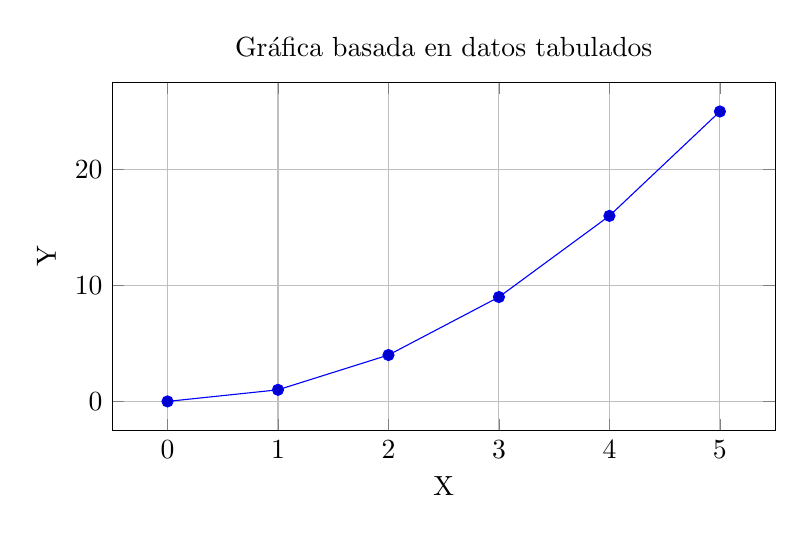
\begin{tikzpicture}
        \begin{axis}[
            title={Gráfica basada en datos tabulados},
            xlabel={X},
            ylabel={Y},
            grid=major, % Añade una cuadrícula mayor
            width=10cm, % Ancho de la gráfica
            height=6cm, % Altura de la gráfica
        ]
        % Datos tabulados para la gráfica
        \addplot table[row sep=\\, y index=1] {
            x y  \\
            0 0  \\
            1 1  \\
            2 4  \\
            3 9  \\
            4 16 \\
            5 25 \\
        };
        \end{axis}
    \end{tikzpicture}
    \caption{Ejemplo de gráfica creada a partir de una tabla de datos}
    \label{fig:tabla_grafica}
\end{figure}
\textbf{\large{\href{https://youtu.be/dQw4w9WgXcQ?si=jGf-LdN459y-xefY}{EJEMPLO DE URL (LINK)}}}
\end{document}